\PassOptionsToPackage{enable-debug,check-declarations}{expl3}
\RequirePackage{pdfmanagement-testphase}
\DeclareDocumentMetadata {  }
\ExplSyntaxOn
\pdfmanagement_add:nnn{Catalog}{Lang}{(enUS)}
\ExplSyntaxOff

% xmp metadata for pdf
% Originally used \usepackage[a-2a]{pdfx}
% \usepackage{hyperxmp} replaced it
% \RequirePackage{pdfmanagement-testphase} replaced it

\documentclass[11pt,
  english,
  letterpaper,
]{article}
\usepackage{sa4ss}
\usepackage{amsmath,amssymb,array}
\usepackage{booktabs}

% From tagged-template.latex
\usepackage{lmodern}
\usepackage{ifxetex,ifluatex}
\ifnum 0\ifxetex 1\fi\ifluatex 1\fi=0 % if pdftex
  \usepackage[T1]{fontenc}
  \usepackage[utf8]{inputenc}
  \usepackage{textcomp} % provide euro and other symbols
\else % if luatex or xetex
  \usepackage{unicode-math}
  \defaultfontfeatures{Scale=MatchLowercase}
  \defaultfontfeatures[\rmfamily]{Ligatures=TeX,Scale=1}
\fi

% Use upquote if available, for straight quotes in verbatim environments
\IfFileExists{upquote.sty}{\usepackage{upquote}}{}
\IfFileExists{microtype.sty}{% use microtype if available
  \usepackage[]{microtype}
  \UseMicrotypeSet[protrusion]{basicmath} % disable protrusion for tt fonts
}{}
\makeatletter
\@ifundefined{KOMAClassName}{% if non-KOMA class
  \IfFileExists{parskip.sty}{%
    \usepackage{parskip}
  }{% else
    \setlength{\parindent}{0pt}
    \setlength{\parskip}{6pt plus 2pt minus 1pt}}
}{% if KOMA class
  \KOMAoptions{parskip=half}}
\makeatother
\usepackage{xcolor}
\IfFileExists{xurl.sty}{\usepackage{xurl}}{} % add URL line breaks if available
\hypersetup{
  pdftitle={Evaluating available information to inform stock management delineation for quillback rockfish (Sebastes maliger) off the U.S. West coast},
  pdflang={en},
  hidelinks,
  pdfcreator={LaTeX via pandoc}}
\urlstyle{same} % disable monospaced font for URLs
\usepackage{longtable}
% Correct order of tables after \paragraph or \subparagraph
\usepackage{etoolbox}
\makeatletter
\patchcmd\longtable{\par}{\if@noskipsec\mbox{}\fi\par}{}{}
\makeatother
% Allow footnotes in longtable head/foot
\IfFileExists{footnotehyper.sty}{\usepackage{footnotehyper}}{\usepackage{footnote}}
\makesavenoteenv{longtable}
\usepackage{graphicx}
\makeatletter
\def\maxwidth{\ifdim\Gin@nat@width>\linewidth\linewidth\else\Gin@nat@width\fi}
\def\maxheight{\ifdim\Gin@nat@height>\textheight\textheight\else\Gin@nat@height\fi}
\makeatother
% Scale images if necessary, so that they will not overflow the page
% margins by default, and it is still possible to overwrite the defaults
% using explicit options in \includegraphics[width, height, ...]{}
\setkeys{Gin}{width=\maxwidth,height=\maxheight,keepaspectratio}
% Set default figure placement to htbp
\makeatletter
\def\fps@figure{htbp}
\makeatother
\setlength{\emergencystretch}{3em} % prevent overfull lines
\providecommand{\tightlist}{%
  \setlength{\itemsep}{0pt}\setlength{\parskip}{0pt}}
\setcounter{secnumdepth}{5}
\ifxetex
  % Load polyglossia as late as possible: uses bidi with RTL langages (e.g. Hebrew, Arabic)
  \usepackage{polyglossia}
  \setmainlanguage[]{english}
\else
  \usepackage[shorthands=off,main=english]{babel}
\fi

%Define cslreferences environment, required by pandoc 2.8
%https://github.com/rstudio/rmarkdown/issues/1649


\providecommand{\tightlist}{%
  \setlength{\itemsep}{0pt}\setlength{\parskip}{0pt}}


\date{}
\newcommand{\trTitle}{Evaluating available information to inform stock management delineation for quillback rockfish (\emph{Sebastes maliger}) off the U.S. West coast}
\newcommand{\trYear}{2021}
\newcommand{\trMonth}{October}
\newcommand{\trAuthsLong}{true}
\newcommand{\trAuthsBack}{Langseth, B.J., C.R. Wetzel}
\newcommand{\trCitation}{
\begin{hangparas}{1em}{1}
\trAuthsBack{}. \trYear{}. \trTitle{}. \glsentrylong{pfmc}, Portland, Oregon. \pageref{LastPage}{}\,p.
\end{hangparas}}

\AtBeginDocument{\tagstructbegin{tag=Document}}
\AtEndDocument{\tagstructend}
\pretocmd{\maketitle}{\tagstructbegin{tag=H1}\tagmcbegin{tag=H1}}{}{}
\apptocmd{\maketitle}{\tagmcend\tagstructend}{}{}

\begin{document}

%%%%% Frontmatter %%%%%

% Footnote symbols in front matter
\renewcommand*{\thefootnote}{\fnsymbol{footnote}}

\small
\thispagestyle{empty}
\pagenumbering{roman}
\noindent
\begin{center}
\title{Evaluating available information to inform stock management delineation for quillback rockfish (\emph{Sebastes maliger}) off the U.S. West coast}
% \textnormal{\MakeTextUppercase{\trTitle{}}}
\vspace{1.5cm}
{\Large\textbf\newline{Evaluating available information to inform stock management delineation for quillback rockfish (\emph{Sebastes maliger}) off the U.S. West coast}}
\vfill
by\\
Brian J. Langseth\textsuperscript{1}\\
Chantel R. Wetzel\textsuperscript{1}\vfill
\textsuperscript{1}Northwest Fisheries Science Center, U.S. Department of Commerce, National Oceanic and Atmospheric Administration, National Marine Fisheries Service, 2725 Montlake Boulevard East, Seattle, Washington 98112\vfill
\trMonth{} \trYear{}
\end{center}
\clearpage

% Fourth page: Colophon
\thispagestyle{empty}
\vspace*{\fill}
\begin{center}
\copyright{} \glsentrylong{pfmc}, \trYear{}\\
\end{center}
\par
\bigskip
\noindent
Correct citation for this publication:
\bigskip
\par
\trCitation{}
\clearpage

% Add TOC to pdf bookmarks (clickable pdf)
\pdfbookmark[1]{\contentsname}{toc}

% Table of contents page, lists of figures and tables
\tableofcontents\clearpage
\label{TRlastRoman}
\clearpage

% Table of contents
\newpage
\thispagestyle{empty} % to remove page number

% Settings for the main document
\pagenumbering{arabic}  % Regular page numbers
\pagestyle{plain}  % No page number on first page of main document, use 'empty'
\renewcommand*{\thefootnote}{\arabic{footnote}}  % Back to numeric footnotes
\setcounter{footnote}{0}  % And start at 1
\renewcommand{\headrulewidth}{0.5pt}
\renewcommand{\footrulewidth}{0.5pt}
%\pagestyle{fancy}\fancyhead[c]{Draft: Do not cite or circulate}

\newcommand{\lt}{\ensuremath <}
\newcommand{\gt}{\ensuremath >}

\pagebreak
\pagenumbering{roman}
\setcounter{page}{1}

\renewcommand{\thetable}{\roman{table}}
\renewcommand{\thefigure}{\roman{figure}}

\setlength\parskip{0.5em plus 0.1em minus 0.2em}

\pagebreak
\setlength{\parskip}{5mm plus1mm minus1mm}
\pagenumbering{arabic}
\setcounter{page}{1}
\renewcommand{\thefigure}{\arabic{figure}}
\renewcommand{\thetable}{\arabic{table}}
\setcounter{table}{0}
\setcounter{figure}{0}

\setlength\parskip{0.2em plus 0.1em minus 0.2em}

\tagstructbegin{tag=H1}\tagmcbegin{tag=H1}

\hypertarget{introduction}{%
\section{Introduction}\label{introduction}}

\leavevmode\tagmcend\tagstructend

\tagstructbegin{tag=P}\tagmcbegin{tag=P}

At the September 2021 Council meeting, the Council requested that the Groundfish Subcommittee (GFSC) evaluate and make recommendations on the stock delineations for copper, quillback, and vermillion/sunset rockfish. Information for copper rockfish was presented at the GFSC mop-up meeting on September 29-30, 2021 ({\tagstructbegin{tag=Reference}\tagmcbegin{tag=Reference}Wetzel (2021)\leavevmode\tagmcend\tagstructend}). This report updates the information prepared on copper rockfish for application to quillback rockfish. There are few directed studies on quillback rockfish compared to copper rockfish so emphasising quillback rockfish adds limited information beyond that already provided for copper rockfish. To more clearly indicate the information most applicable to quillback rockfish, we have added text to the beginning of the study descriptions to clarify studies that focus on or include quillback rockfish.

\leavevmode\tagmcend\tagstructend\par

\tagstructbegin{tag=H1}\tagmcbegin{tag=H1}

\hypertarget{status-determination-across-area-based-assessments}{%
\section{Status determination across area-based assessments}\label{status-determination-across-area-based-assessments}}

\leavevmode\tagmcend\tagstructend

\tagstructbegin{tag=H2}\tagmcbegin{tag=H2}

\hypertarget{dispersal}{%
\subsection{Dispersal}\label{dispersal}}

\leavevmode\tagmcend\tagstructend

\tagstructbegin{tag=H3}\tagmcbegin{tag=H3}

\hypertarget{recruitment-and-dispersal}{%
\subsubsection{Recruitment and Dispersal}\label{recruitment-and-dispersal}}

\leavevmode\tagmcend\tagstructend

\tagstructbegin{tag=P}\tagmcbegin{tag=P}

\emph{Evidence for Managing at Assessment Scale}

\leavevmode\tagmcend\tagstructend\par

\tagstructbegin{tag=P}\tagmcbegin{tag=P}

Markel {\tagstructbegin{tag=Reference}\tagmcbegin{tag=Reference}(2011)\leavevmode\tagmcend\tagstructend} - quillback included: Observed significant differences of recruitment among sites and years which were not consistent, indicating spatial differences in recruitment intensity during year of high recruitment within the Barkley Sound, British Columbia. Study was based on black rockfish, and a complex of copper, quillback, and brown rockfish.

\leavevmode\tagmcend\tagstructend\par

\tagstructbegin{tag=P}\tagmcbegin{tag=P}

Buonaccorsi et al.~{\tagstructbegin{tag=Reference}\tagmcbegin{tag=Reference}(2004)\leavevmode\tagmcend\tagstructend} - no quillback: Estimated the dispersal distance of copper rockfish recruits as 13km or less, and dispersal distance of grass rockfish recruits as 11km or less, based on a stepping stone model. \emph{Caveat}: These values can be highly sensitive to the ratio of total population size to effective population size.

\leavevmode\tagmcend\tagstructend\par

\tagstructbegin{tag=P}\tagmcbegin{tag=P}

Wilson et al.~{\tagstructbegin{tag=Reference}\tagmcbegin{tag=Reference}(2008)\leavevmode\tagmcend\tagstructend} - no quillback: Found greater correlation of recruitment strength with localized environmental conditions than with regional environmental patterns in California for kelp, copper, gopher, and black and yellow rockfish. \emph{Caveat}: Limited regional variability during time of study was identified as possible reason for limited correlation between regional environmental patterns and recruitment.

\leavevmode\tagmcend\tagstructend\par

\tagstructbegin{tag=P}\tagmcbegin{tag=P}

Sivasundar and Palumbi {\tagstructbegin{tag=Reference}\tagmcbegin{tag=Reference}(2010)\leavevmode\tagmcend\tagstructend} - no quillback: Have a schematic (their Figure 1) that shows a general ecological gradient from weak upwelling and high larval settlement in waters off Oregon/Washington to strong upwelling and low larval settlement in waters near Point Conception, California.

\leavevmode\tagmcend\tagstructend\par

\tagstructbegin{tag=P}\tagmcbegin{tag=P}

\emph{Evidence for Alternative Management Scale}

\leavevmode\tagmcend\tagstructend\par

\tagstructbegin{tag=P}\tagmcbegin{tag=P}

Field et al.~{\tagstructbegin{tag=Reference}\tagmcbegin{tag=Reference}(2021)\leavevmode\tagmcend\tagstructend} - no quillback: Determined that rockfish strong recruitments observed between 2014-2016 were largely coastwide events. \emph{Caveat}: study utilizes a large dataset covering a wide spatial and temporal range, although neither copper nor quillback were among the most caught species.

\leavevmode\tagmcend\tagstructend\par

\tagstructbegin{tag=P}\tagmcbegin{tag=P}

\emph{Information from assessment reports}

\leavevmode\tagmcend\tagstructend\par

\tagstructbegin{tag=P}\tagmcbegin{tag=P}

Annual recruitment deviations were estimated in the base models for California and Oregon, but not Washington. Overlaying recruitment estimates across areas (using the model sensitivity to estimating annual recruitment deviations for Washington) showed some general coherence with the overall patterns of positive or negative recruitment deviations among areas, with variability in individual years (Figure \ref{fig:recruit-comparison}). In the base model for Washington we opted to not estimate annual recruitment deviations due to limited information available in the length compositions for that area). \emph{Caveat}: Length data may not be fully informative for recruitment as variation in growth can result in low or high recruitment years being attributed to multiple years.

\leavevmode\tagmcend\tagstructend\par

\tagstructbegin{tag=Figure,alttext={.}}\tagmcbegin{tag=Figure}

\begin{figure}
\centering
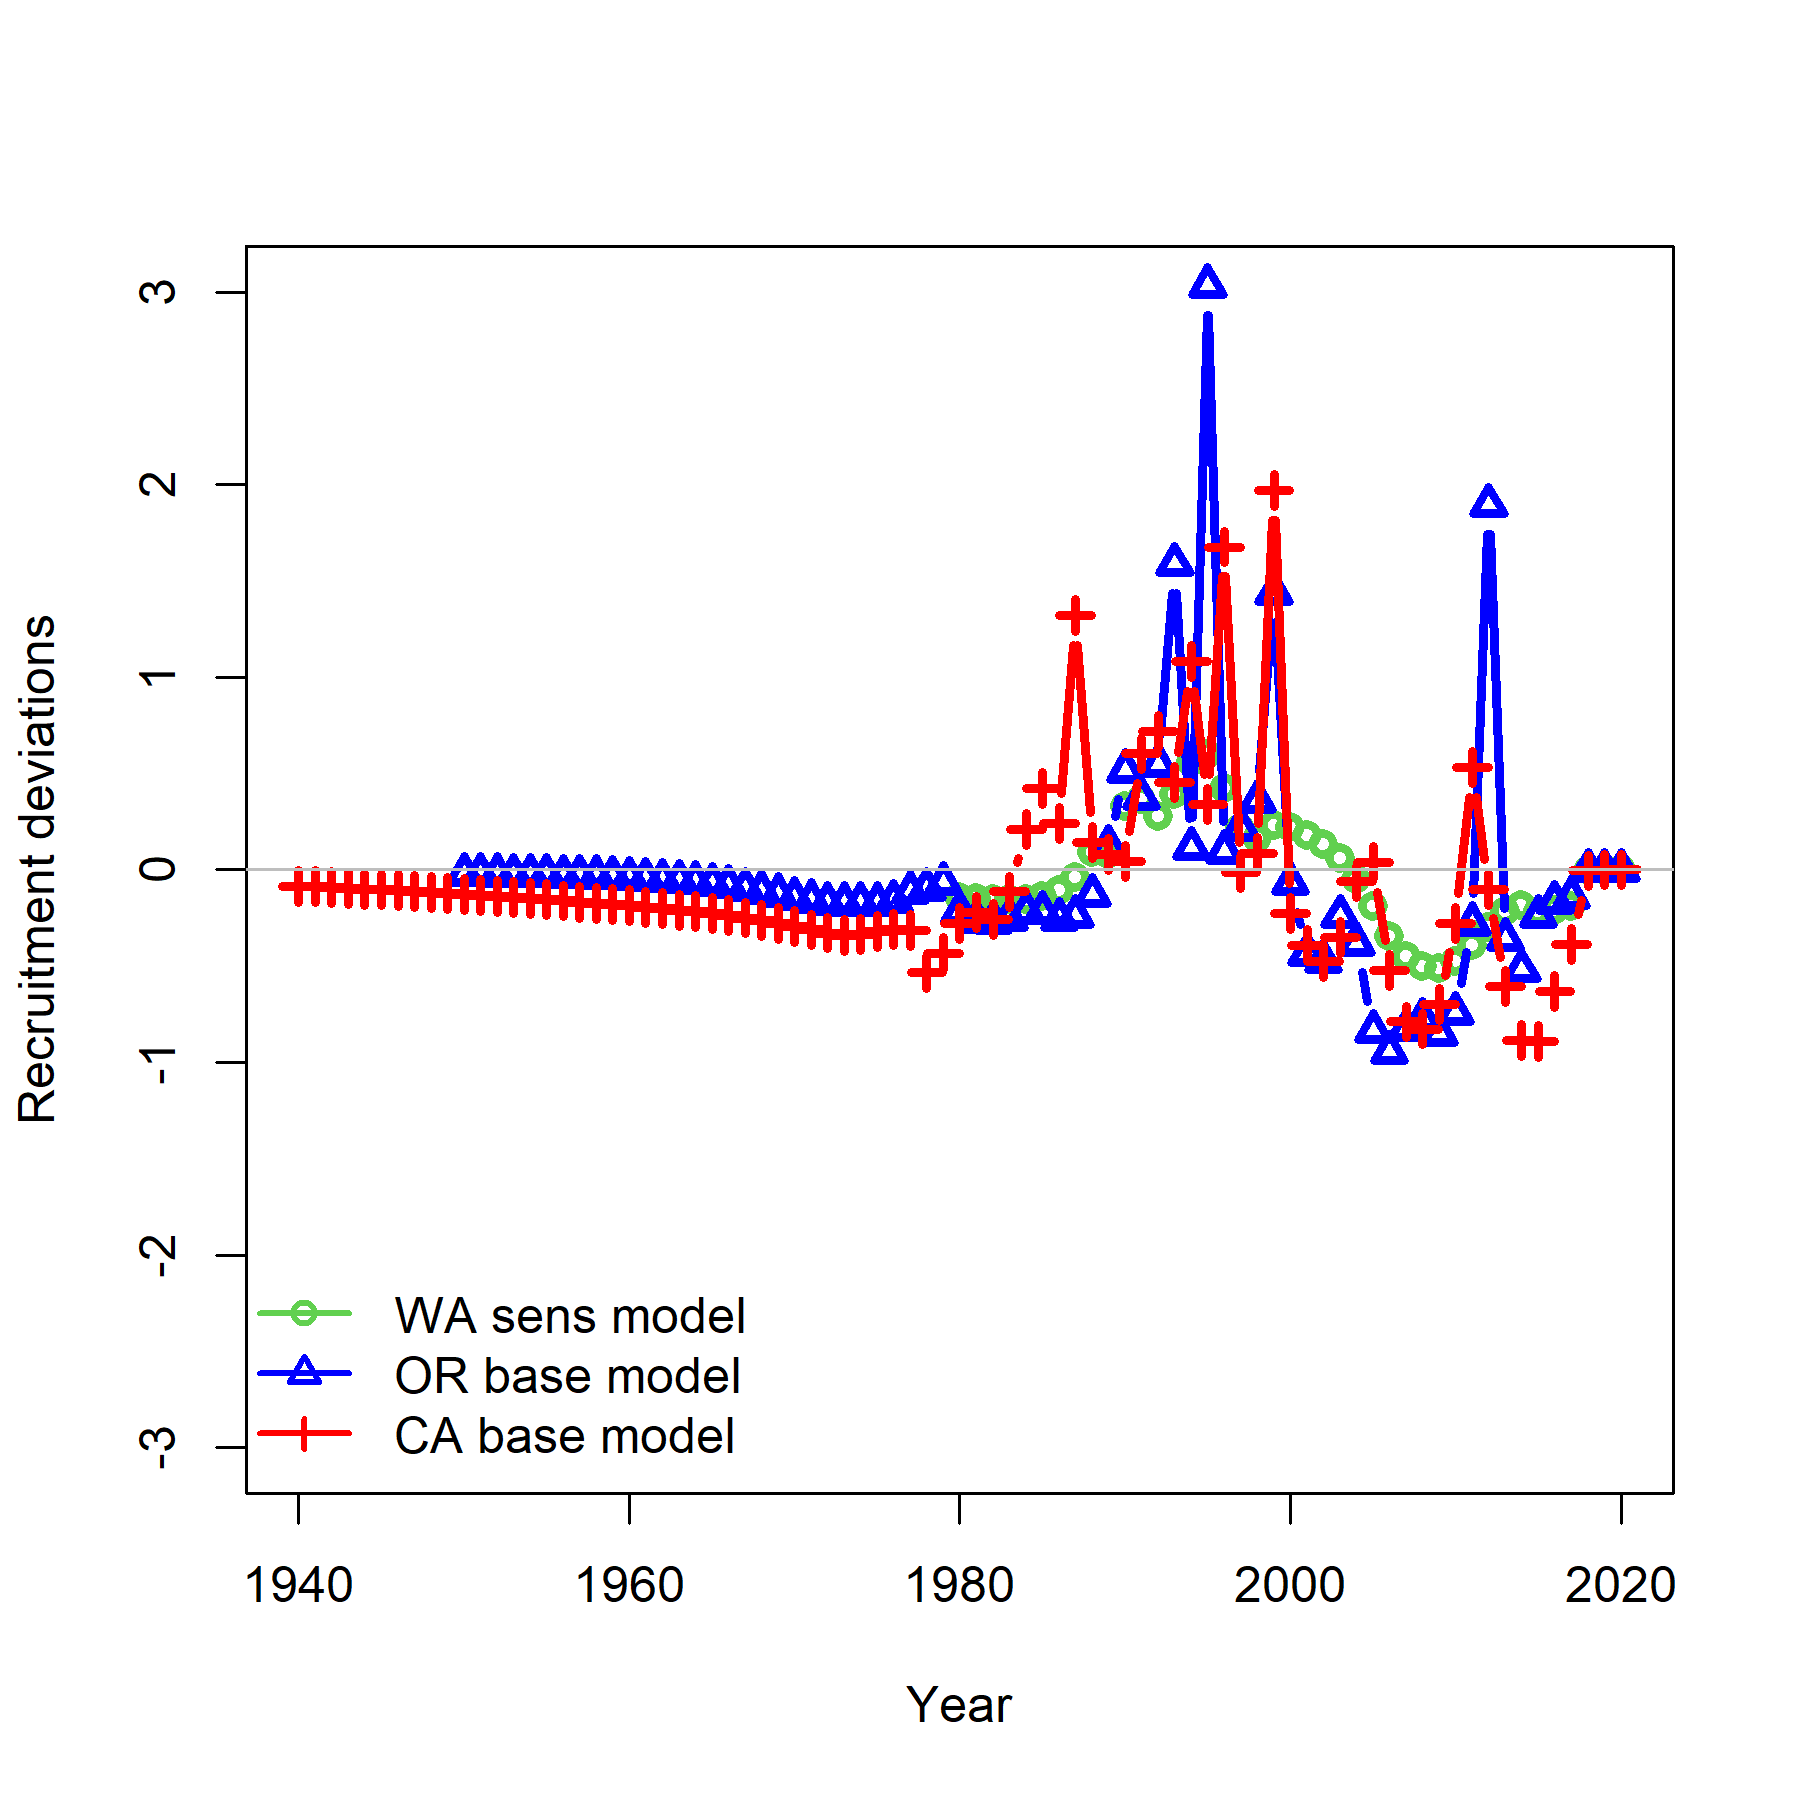
\includegraphics[width=1\textwidth,height=1\textheight]{comprare_recruitments.png}
\caption{Estimates of recruitment in millions of eggs from the base models for Oregon and California, and from the sensitivity where recruitment was estimated for Washington.\label{fig:recruit-comparison}}
\end{figure}

\tagmcend\tagstructend

\tagstructbegin{tag=H3}\tagmcbegin{tag=H3}

\hypertarget{adult-movement}{%
\subsubsection{Adult Movement}\label{adult-movement}}

\leavevmode\tagmcend\tagstructend

\tagstructbegin{tag=P}\tagmcbegin{tag=P}

\emph{Evidence for Managing at Assessment Scale}

\leavevmode\tagmcend\tagstructend\par

\tagstructbegin{tag=P}\tagmcbegin{tag=P}

Lea et al {\tagstructbegin{tag=Reference}\tagmcbegin{tag=Reference}(1999)\leavevmode\tagmcend\tagstructend} - quillback mentioned: Summarized tagging data from Moro to Monterey Bay, California that reported species of the gopher complex (which includes quillback rockfish though no quillback rockfish data were provided) to have no movement and therefore considered very residential in California. Copper rockfish was found to have limited movement; of 32 tagged copper that were recaptured the distance moved ranged between 0-1.5 nautical miles after 2-1,017 days at liberty.

\leavevmode\tagmcend\tagstructend\par

\tagstructbegin{tag=P}\tagmcbegin{tag=P}

Matthews {\tagstructbegin{tag=Reference}\tagmcbegin{tag=Reference}(1990b)\leavevmode\tagmcend\tagstructend} - quillback focus: Home ranges of four tagged quillback and 11 tagged copper rockfish in Puget Sound, Washington were \textless10km{\tagstructbegin{tag=Formula}\tagmcbegin{tag=Formula}\(^2\)\leavevmode\tagmcend\tagstructend} on high relief reefs but greater (4000km{\tagstructbegin{tag=Formula}\tagmcbegin{tag=Formula}\(^2\)\leavevmode\tagmcend\tagstructend}) on low relief reefs. Additional , home ranges exhibited long periods of residency with limited movements. A study with substantially more samples based on copper, quillback, and brown rockfish {\tagstructbegin{tag=Reference}\tagmcbegin{tag=Reference}(Matthews 1990a)\leavevmode\tagmcend\tagstructend} indicated similar patterns with ranges from 8km{\tagstructbegin{tag=Formula}\tagmcbegin{tag=Formula}\(^2\)\leavevmode\tagmcend\tagstructend}-1500km{\tagstructbegin{tag=Formula}\tagmcbegin{tag=Formula}\(^2\)\leavevmode\tagmcend\tagstructend} depending on reef type and season.

\leavevmode\tagmcend\tagstructend\par

\tagstructbegin{tag=P}\tagmcbegin{tag=P}

Tolimieri et al.~{\tagstructbegin{tag=Reference}\tagmcbegin{tag=Reference}(2009)\leavevmode\tagmcend\tagstructend} - quillback included: Observed home ranges of quillback rockfish in Puget Sound, Washington was relatively small (\textasciitilde1500 to \textasciitilde2500m{\tagstructbegin{tag=Formula}\tagmcbegin{tag=Formula}\(^2\)\leavevmode\tagmcend\tagstructend}) and similar among copper and quillback rockfish and lingcod. Caveat: movement of fish in the Puget Sound may not be representative of movement in coastal populations.

\leavevmode\tagmcend\tagstructend\par

\tagstructbegin{tag=P}\tagmcbegin{tag=P}

Hannah and Rankin {\tagstructbegin{tag=Reference}\tagmcbegin{tag=Reference}(2011)\leavevmode\tagmcend\tagstructend} - quillback focused: Observed high site fidelity for quillback rockfish based on tagging of four individuals tracked for approximately one year. Quillback rockfish exhibited higher site fidelity than copper rockfish.

\leavevmode\tagmcend\tagstructend\par

\tagstructbegin{tag=P}\tagmcbegin{tag=P}

\emph{Evidence for Alternative Management Scale}

\leavevmode\tagmcend\tagstructend\par

\tagstructbegin{tag=P}\tagmcbegin{tag=P}

Lowe et al.~{\tagstructbegin{tag=Reference}\tagmcbegin{tag=Reference}(2009)\leavevmode\tagmcend\tagstructend} - no quillback: Copper rockfish exhibited low degrees of site fidelity and had high variation in the percentage of days on which individuals were detected based on 7 tagged fish at petroleum platforms in the Santa Barbara Channel.

\leavevmode\tagmcend\tagstructend\par

\tagstructbegin{tag=P}\tagmcbegin{tag=P}

McGilliard et al.~{\tagstructbegin{tag=Reference}\tagmcbegin{tag=Reference}(2015)\leavevmode\tagmcend\tagstructend} - general: Fisheries managed by area closures impose spatial heterogeneity in fishing mortality, and simulations from generic operating models suggest that the accuracy of conventional stock assessments depends on movement rates.

\leavevmode\tagmcend\tagstructend\par

\tagstructbegin{tag=H2}\tagmcbegin{tag=H2}

\hypertarget{geographic-variation}{%
\subsection{Geographic variation}\label{geographic-variation}}

\leavevmode\tagmcend\tagstructend

\tagstructbegin{tag=H3}\tagmcbegin{tag=H3}

\hypertarget{variation-in-genetic-composition}{%
\subsubsection{Variation in Genetic Composition}\label{variation-in-genetic-composition}}

\leavevmode\tagmcend\tagstructend

\tagstructbegin{tag=P}\tagmcbegin{tag=P}

There are very limited genetic studies available for quillback rockfish along U.S. West Coast

\leavevmode\tagmcend\tagstructend\par

\tagstructbegin{tag=P}\tagmcbegin{tag=P}

\emph{Evidence for Managing at Assessment Scale}

\leavevmode\tagmcend\tagstructend\par

\tagstructbegin{tag=P}\tagmcbegin{tag=P}

Sivasundar and Palumbi {\tagstructbegin{tag=Reference}\tagmcbegin{tag=Reference}(2010)\leavevmode\tagmcend\tagstructend} - no quillback: Measured moderate differentiation in mtDNA structure but no nuclear structure in coastal copper rockfish populations. \emph{Caveat}: other species that were included in this analysis had a mix of differentiation and no differentiation.

\leavevmode\tagmcend\tagstructend\par

\tagstructbegin{tag=P}\tagmcbegin{tag=P}

Buonaccorsi et al.~{\tagstructbegin{tag=Reference}\tagmcbegin{tag=Reference}(2002)\leavevmode\tagmcend\tagstructend} - no quillback: Identified significant divergence along the U.S. West Coast when measured as variance in allele frequency or mean repeat number, indicting a substantial isolation by distance between regions. Examined samples from Queen Charlotte, Puget Sound, Canadian Gulf Islands, Crescent City, Big Creek, San Miguel Island.

\leavevmode\tagmcend\tagstructend\par

\tagstructbegin{tag=P}\tagmcbegin{tag=P}

Johansson et al.~{\tagstructbegin{tag=Reference}\tagmcbegin{tag=Reference}(2008)\leavevmode\tagmcend\tagstructend} - no quillback: Identified isolation by distance in coastal copper rockfish populations ({\tagstructbegin{tag=Formula}\tagmcbegin{tag=Formula}\(\text{F}_\text{ST}\)\leavevmode\tagmcend\tagstructend} = 0.006) similar to Buonaccorsi et al.~{\tagstructbegin{tag=Reference}\tagmcbegin{tag=Reference}(2002)\leavevmode\tagmcend\tagstructend} ({\tagstructbegin{tag=Formula}\tagmcbegin{tag=Formula}\(\text{F}_\text{ST}\)\leavevmode\tagmcend\tagstructend} = 0.008). However, concluded that some of the genetic divergence may be related to habitat patchiness and not distance alone.

\leavevmode\tagmcend\tagstructend\par

\tagstructbegin{tag=P}\tagmcbegin{tag=P}

\emph{Evidence for Alternative Management Scale}

\leavevmode\tagmcend\tagstructend\par

\tagstructbegin{tag=P}\tagmcbegin{tag=P}

Sivasundar and Palumbi {\tagstructbegin{tag=Reference}\tagmcbegin{tag=Reference}(2010)\leavevmode\tagmcend\tagstructend} - no quillback: The Oregon and Monterey Bay populations were both genetically differentiated from the Santa Barbara populations for mtDNA but the Monterey Bay and Oregon populations could not be distinguished from each other. This could indicate that there is limited differentiation between northern California and Oregon copper rockfish populations indicating mixing between the areas.

\leavevmode\tagmcend\tagstructend\par

\tagstructbegin{tag=P}\tagmcbegin{tag=P}

Seeb {\tagstructbegin{tag=Reference}\tagmcbegin{tag=Reference}(1998)\leavevmode\tagmcend\tagstructend} - quillback focused: Significant genetic differences were found between Puget Sound and coastal stocks of quillback rockfish based on allozyme frequency and mtDNA, however there was not significant differentiation in allozyme frequency in populations of quillback rockfish between coastal Washington and Alaska.

\leavevmode\tagmcend\tagstructend\par

\tagstructbegin{tag=P}\tagmcbegin{tag=P}

\emph{Caveat}

\leavevmode\tagmcend\tagstructend\par

\tagstructbegin{tag=P}\tagmcbegin{tag=P}

Waples and Gaggiotti {\tagstructbegin{tag=Reference}\tagmcbegin{tag=Reference}(2006)\leavevmode\tagmcend\tagstructend}: Significant differences in neutral genetic characters indicate that the populations have been reproductively isolated for many generations, which is far longer than the ecological time scales that are relevant to stock assessment or fishery management. Argue for use of mtDNA data to determine demographic independence on the scales relevant to stock assessment.

\leavevmode\tagmcend\tagstructend\par

\tagstructbegin{tag=P}\tagmcbegin{tag=P}

Schwenke et al.~{\tagstructbegin{tag=Reference}\tagmcbegin{tag=Reference}(2018)\leavevmode\tagmcend\tagstructend} - quillback included: Found long-term low-level introgression among quillback, copper, and brown rockfish within the Salish sea at higher rates than in coastal populations. Suggests greater isolation of Salish Sea populations, possibly due to the specific environmental conditions in the sub basins of the Salish Sea.

\leavevmode\tagmcend\tagstructend\par

\tagstructbegin{tag=P}\tagmcbegin{tag=P}

Stout et al.~{\tagstructbegin{tag=Reference}\tagmcbegin{tag=Reference}(2001)\leavevmode\tagmcend\tagstructend} - quillback focused: Concluded there were three distinct population sub-units within Puget Sound, Washington. Relied heavily on information from the genetic studies of Seeb {\tagstructbegin{tag=Reference}\tagmcbegin{tag=Reference}(1998)\leavevmode\tagmcend\tagstructend}.

\leavevmode\tagmcend\tagstructend\par

\tagstructbegin{tag=H3}\tagmcbegin{tag=H3}

\hypertarget{variation-in-phenotypic-traits}{%
\subsubsection{Variation in Phenotypic Traits}\label{variation-in-phenotypic-traits}}

\leavevmode\tagmcend\tagstructend

\tagstructbegin{tag=P}\tagmcbegin{tag=P}

\emph{Evidence for Managing at Assessment Scale}

\leavevmode\tagmcend\tagstructend\par

\tagstructbegin{tag=P}\tagmcbegin{tag=P}

Minor differences measured in maturity-at-length between two areas of the coast for copper rockfish: Oregon {\tagstructbegin{tag=Reference}\tagmcbegin{tag=Reference}(Hannah 2014)\leavevmode\tagmcend\tagstructend} and South of Point Conception (Melissa Head, NWFSC). \emph{Caveat}: Maturity data for quillback rockfish was only available for Oregon samples {\tagstructbegin{tag=Reference}\tagmcbegin{tag=Reference}(Robert W. Hannah and Blume 2011)\leavevmode\tagmcend\tagstructend} so coastal comparisons were not available.

\leavevmode\tagmcend\tagstructend\par

\tagstructbegin{tag=P}\tagmcbegin{tag=P}

Punt et al.{\tagstructbegin{tag=Reference}\tagmcbegin{tag=Reference}(2015)\leavevmode\tagmcend\tagstructend} - general: Conventional stock assessments produced significantly biased estimates when applied to an operating model of pink ling fisheries with spatial heterogeneity in fishing mortality, growth, and recruitment.

\leavevmode\tagmcend\tagstructend\par

\tagstructbegin{tag=P}\tagmcbegin{tag=P}

\emph{Evidence for Alternative Management Scale}

\leavevmode\tagmcend\tagstructend\par

\tagstructbegin{tag=P}\tagmcbegin{tag=P}

Limited differences in growth based on original age-length estimates between fish off the Oregon and Washington coast were shown at data workshop in October, 2020. Limited number of new California samples during reviews considered insufficient to estimate a California curve for comparison. Stock assessments used a single coastwide growth curve. \emph{Caveat}: Spatial gradients of growth across the coast are commonly observed in rockfish or other fish species along the U.S. west coast {\tagstructbegin{tag=Reference}\tagmcbegin{tag=Reference}(Keller et al. 2012, 2018; Gertseva, Matson, and Cope 2017)\leavevmode\tagmcend\tagstructend}.

\leavevmode\tagmcend\tagstructend\par

\tagstructbegin{tag=P}\tagmcbegin{tag=P}

The assessments for quillback rockfish utilized the same growth, maturity, fecundity, and length-weight relationships across areas.

\leavevmode\tagmcend\tagstructend\par

\tagstructbegin{tag=H2}\tagmcbegin{tag=H2}

\hypertarget{other-considerations}{%
\subsection{Other Considerations}\label{other-considerations}}

\leavevmode\tagmcend\tagstructend

\tagstructbegin{tag=H3}\tagmcbegin{tag=H3}

\hypertarget{abundance-trends}{%
\subsubsection{Abundance Trends}\label{abundance-trends}}

\leavevmode\tagmcend\tagstructend

\tagstructbegin{tag=P}\tagmcbegin{tag=P}

\emph{Evidence for Managing at Assessment Scale}

\leavevmode\tagmcend\tagstructend\par

\tagstructbegin{tag=P}\tagmcbegin{tag=P}

Ying et al.~{\tagstructbegin{tag=Reference}\tagmcbegin{tag=Reference}(2011)\leavevmode\tagmcend\tagstructend}: Measured the performance of stock assessments using an operating model to represent three connected sub-populations of small yellow croaker and observed that assessing and managing each sub-population as a unit led to overfishing and managing the metapopulation as a unit stock often led to local depletion.

\leavevmode\tagmcend\tagstructend\par

\tagstructbegin{tag=P}\tagmcbegin{tag=P}

The trajectories across all model areas showed varying patterns (Figure \ref{fig:relb-comparison}). The separate models for the modeled areas estimated different stock trajectories with the stock in California declining earlier, and to a greater degree, than in Oregon or Washington. Both Oregon and California display an increase in stock size starting in the early 2000s that differs in the magnitude of increase, while Washington's change in stock size is much more gradual overall, and seemingly opposite to that of Oregon and California in recent years. The model for Washington did not estimate annual recruitment deviations which likely contributes to stock trajectory differences in recent years (where large recruitment pulses in the 1990s led to increases in recent stock size).

\leavevmode\tagmcend\tagstructend\par

\tagstructbegin{tag=Figure,alttext={.}}\tagmcbegin{tag=Figure}

\begin{figure}
\centering
\includegraphics[width=1\textwidth,height=1\textheight]{L:/Assessments/CurrentAssessments/DataModerate_2021/Quillback_Rockfish/presentations/base_comparisonscompare4_Bratio_uncertainty.png}
\caption{Estimated relative spawning output (in millions of eggs) by assessed area.\label{fig:relb-comparison}}
\end{figure}

\tagmcend\tagstructend

\clearpage

\tagstructbegin{tag=P}\tagmcbegin{tag=P}

\emph{Evidence for Alternative Management Scale}

\leavevmode\tagmcend\tagstructend\par

\tagstructbegin{tag=P}\tagmcbegin{tag=P}

The areas of true population variation in relative stock size may not align with the assessment boundaries as currently defined. State based management is likely not the only factor impacting relative stock sizes across the coast where movement, habitat availability, and recruitment patterns likely also influence potential differences in relative stock size.

\leavevmode\tagmcend\tagstructend\par

\tagstructbegin{tag=P}\tagmcbegin{tag=P}

\emph{Caveat}

\leavevmode\tagmcend\tagstructend\par

\tagstructbegin{tag=P}\tagmcbegin{tag=P}

Cope and Punt {\tagstructbegin{tag=Reference}\tagmcbegin{tag=Reference}(2013)\leavevmode\tagmcend\tagstructend}: Conventional stock assessments failed to estimate differing spatial patterns and exploitation (localized depletion) but adequately estimated the overall stock status. These findings are supported by Bosley et al.~{\tagstructbegin{tag=Reference}\tagmcbegin{tag=Reference}(2021)\leavevmode\tagmcend\tagstructend} who found parameter estimates were generally unbiased at the system level but biased for sub-areas when assumptions about the spatial structure of the population were incorrect.

\leavevmode\tagmcend\tagstructend\par

\tagstructbegin{tag=P}\tagmcbegin{tag=P}

Bosley et al.~{\tagstructbegin{tag=Reference}\tagmcbegin{tag=Reference}(2021)\leavevmode\tagmcend\tagstructend} also found via simulation that spatial estimation models were generally more robust (i.e.~bias was lower) than assuming non-spatial dynamics, even when the underlying spatial structure of the population was unknown or not present.

\leavevmode\tagmcend\tagstructend\par

\tagstructbegin{tag=H3}\tagmcbegin{tag=H3}

\hypertarget{size-and-age-composition}{%
\subsubsection{Size and Age Composition}\label{size-and-age-composition}}

\leavevmode\tagmcend\tagstructend

\tagstructbegin{tag=P}\tagmcbegin{tag=P}

\emph{Evidence for Managing at Assessment Scale}

\leavevmode\tagmcend\tagstructend\par

\tagstructbegin{tag=P}\tagmcbegin{tag=P}

Different selectivity curves were estimated between the recreational and commercial fisheries across modeled areas (Figure \ref{fig:selectivity-comparison}). Differences were greater between Oregon and California recreational selectivity than Oregon and Washington. For commercial selectivity, the size at which quillback rockfish began to be selected was similar for Oregon and Washington, but the slope of the selectivity curve was similar for California and Washington.

\leavevmode\tagmcend\tagstructend\par

\tagstructbegin{tag=Figure,alttext={.}}\tagmcbegin{tag=Figure}

\begin{figure}
\centering
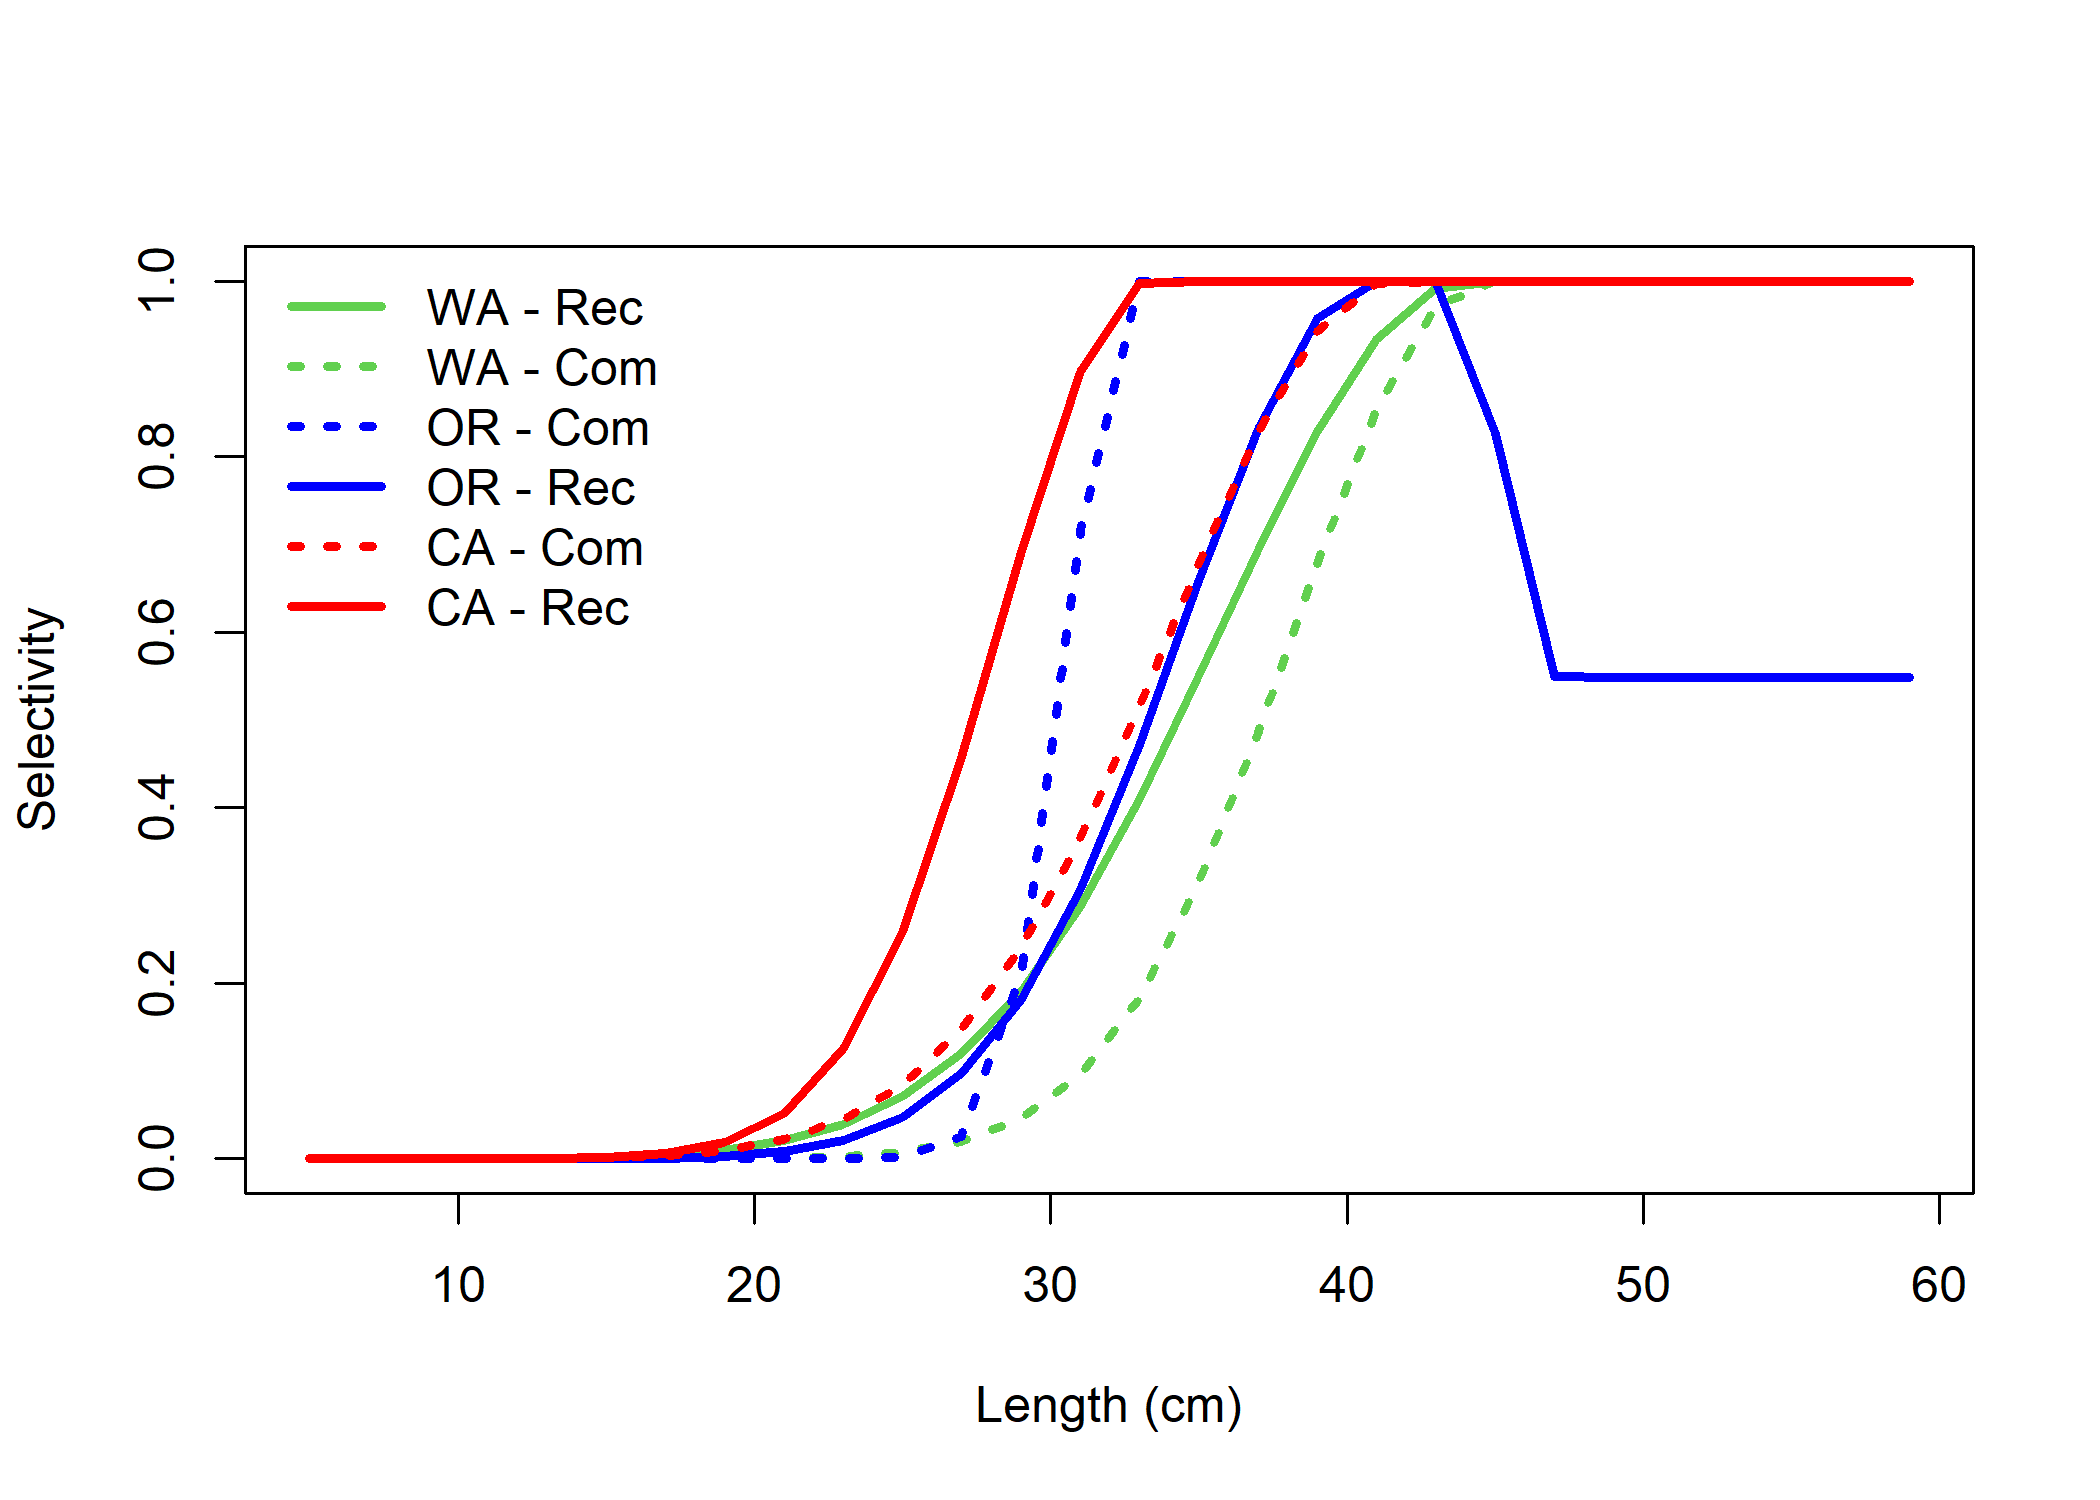
\includegraphics[width=1\textwidth,height=1\textheight]{comprare_selectivity.png}
\caption{Estimated selectivity patterns for commercial (dashed line) and recreational (solid line) fleets by assessed area.\label{fig:selectivity-comparison}}
\end{figure}

\tagmcend\tagstructend

\clearpage

\tagstructbegin{tag=P}\tagmcbegin{tag=P}

Bosely et al.~{\tagstructbegin{tag=Reference}\tagmcbegin{tag=Reference}(2019)\leavevmode\tagmcend\tagstructend}: Specifying the correct form of spatial population structure may not be as critical as understanding movement patterns and spatial heterogeneity in fishery selectivity and life-history variation when developing reference points for management.

\leavevmode\tagmcend\tagstructend\par

\tagstructbegin{tag=P}\tagmcbegin{tag=P}

Berger et al.~{\tagstructbegin{tag=Reference}\tagmcbegin{tag=Reference}(2021)\leavevmode\tagmcend\tagstructend}: Aligning management assessment areas with with underlying population structure and processes is important, especially when fishing mortality is disproportionate to vulnerable biomass among management areas, demographic parameters (growth and maturity) are not homogeneous within management areas, and connectivity (via recruitment or movement) unknowingly exists among management areas. Bias and risk were greater for assessments that incorrectly span multiple population segments compared to assessments that cover a subset of a population segment, and these results were exacerbated when there was connectivity between population segments. \emph{Caveat}: The variation in growth and connectivity between areas via recruitment for quillback rockfish off the West Coast is currently unknown or uncertain.

\leavevmode\tagmcend\tagstructend\par

\tagstructbegin{tag=P}\tagmcbegin{tag=P}

\emph{Caveat}

\leavevmode\tagmcend\tagstructend\par

\tagstructbegin{tag=P}\tagmcbegin{tag=P}

Rather than creating separate assessments to account for variation in exploitation or life-history variation across areas a more integrated approach could be to apply a spatial assessment that can provide both area- and coastwide population estimates. However, spatial assessments come at the cost of a larger number of parameters to estimate, but general guidance around the key decisions exists when moving to spatial assessments (Punt {\tagstructbegin{tag=Reference}\tagmcbegin{tag=Reference}(2019)\leavevmode\tagmcend\tagstructend}). This approach should be evaluated to understand the trade-offs between adding parameters that may be poorly informed (e.g., movement, recruitment by area) via a spatial assessment approach versus either conducting separate assessments or applying the ``fleets-as-areas'' approach.

\leavevmode\tagmcend\tagstructend\par

\clearpage

\clearpage

\tagstructbegin{tag=H1}\tagmcbegin{tag=H1}

\hypertarget{references}{%
\section{References}\label{references}}

\leavevmode\tagmcend\tagstructend

\tagstructbegin{tag=BibEntry}\tagmcbegin{tag=BibEntry}

\hypertarget{refs}{}
\leavevmode\hypertarget{ref-berger_incoherent_2021}{}%
Berger, Aaron M, Jonathan J Deroba, Katelyn M Bosley, Daniel R Goethel, Brian J Langseth, Amy M Schueller, and Dana H Hanselman. 2021. ``Incoherent Dimensionality in Fisheries Management: Consequences of Misaligned Stock Assessment and Population Boundaries.'' Edited by Valerio Bartolino. \emph{ICES Journal of Marine Science} 78 (1): 155--71. \url{https://doi.org/10.1093/icesjms/fsaa203}.

\leavevmode\hypertarget{ref-bosley_overcoming_2019}{}%
Bosley, Katelyn M., Daniel R. Goethel, Aaron M. Berger, Jonathan J. Deroba, Kari H. Fenske, Dana H. Hanselman, Brian J. Langseth, and Amy M. Schueller. 2019. ``Overcoming Challenges of Harvest Quota Allocation in Spatially Structured Populations.'' \emph{Fisheries Research} 220 (December): 105344. \url{https://doi.org/10.1016/j.fishres.2019.105344}.

\leavevmode\hypertarget{ref-Bosleyetal_mismatch_2021}{}%
Bosley, Katelyn M., Amy M. Schueller, Daniel R. Goethel, Dana H. Hanselman, Kari H. Fenske, Aaron M. Berger, Jonathan J. Deroba, and Brian J. Langseth. 2021. ``Finding the Perfect Mismatch: Evaluating Misspecification of Population Structure Within Spatially Explicit Integrated Population Models.'' \emph{Fish and Fisheries} n/a (n/a). \url{https://doi.org/https://doi.org/10.1111/faf.12616}.

\leavevmode\hypertarget{ref-buonaccorsi_population_2002}{}%
Buonaccorsi, Vincent P, Carol A Kimbrell, Eric A Lynn, and Russell D Vetter. 2002. ``Population Structure of Copper Rockfish (\emph{Sebastes Caurinus}) Reflects Postglacial Colonization and Contemporary Patterns of Larval Dispersal.'' \emph{Canadian Journal of Fisheries and Aquatic Sciences} 59 (8): 1374--84. \url{https://doi.org/10.1139/f02-101}.

\leavevmode\hypertarget{ref-buonaccorsi_molecular_2004}{}%
Buonaccorsi, V. P., M. Westerman, J. Stannard, C. Kimbrell, E. Lynn, and R. D. Vetter. 2004. ``Molecular Genetic Structure Suggests Limited Larval Dispersal in Grass Rockfish, Sebastes Rastrelliger.'' \emph{Marine Biology} -1 (1): 1--1. \url{https://doi.org/10.1007/s00227-004-1362-2}.

\leavevmode\hypertarget{ref-cope_data-moderate_2013}{}%
Cope, Jason, E. J. Dick, Alec MacCall, Melissa Monk, Braden Soper, and Chantel Wetzel. 2013. ``Data-Moderate Stock Assessments for Brown, China, Copper, Sharpchin, Stripetail, and Yellowtail Rockfishes and English and Rex Soles in 2013.'' 7700 Ambassador Place NE, Suite 200, Portland, OR: Pacific Fishery Management Council. \url{http://www.academia.edu/download/44999856/CopeetalDataModerate2013.pdf}.

\leavevmode\hypertarget{ref-field_spatiotemporal_2021}{}%
Field, John C., Rebecca R. Miller, Jarrod A. Santora, Nick Tolimieri, Melissa A. Haltuch, Richard D. Brodeur, Toby D. Auth, et al. 2021. ``Spatiotemporal Patterns of Variability in the Abundance and Distribution of Winter-Spawned Pelagic Juvenile Rockfish in the California Current.'' Edited by Geir Ottersen. \emph{PLOS ONE} 16 (5): e0251638. \url{https://doi.org/10.1371/journal.pone.0251638}.

\leavevmode\hypertarget{ref-gertseva_spatial_2017}{}%
Gertseva, Vladlena, Sean E. Matson, and Jason Cope. 2017. ``Spatial Growth Variability in Marine Fish: Example from Northeast Pacific Groundfish.'' Edited by Emory Anderson. \emph{ICES Journal of Marine Science} 74 (6): 1602--13. \url{https://doi.org/10.1093/icesjms/fsx016}.

\leavevmode\hypertarget{ref-hannah_length_2014}{}%
Hannah, Robert W. 2014. ``Length and Age at Maturity of Female Copper Rockfish (\emph{Sebastes Caurinus}) from Oregon Waters Based on Histological Evaluation of Ovaries.'' Information Reports 2014-04. Oregon Department of Fish; Wildlife.

\leavevmode\hypertarget{ref-HannahandBlume_maturity_2011}{}%
Hannah, Robert W., and Matthew T. O. Blume. 2011. ``Maturity of Female Quillback (\emph{Sebastes Maliger}) and China Rockfish (\emph{S. Nebulosus}) from Oregon Waters Based on Histological Evaluation of Ovaries.'' Information Reports 2011-01. Oregon Department of Fish; Wildlife.

\leavevmode\hypertarget{ref-HannahandRankin_rockfish_site_fidelity_2011}{}%
Hannah, Robert W., and Polly S. Rankin. 2011. ``Site Fidelity and Movement of Eight Species of Pacific Rockfish at a High-Relief Rocky Reef on the Oregon Coast.'' \emph{North American Journal of Fisheries Management} 31: 483--94.

\leavevmode\hypertarget{ref-johansson_influence_2008}{}%
Johansson, M. L., M. A. Banks, K. D. Glunt, H. M. Hassel-Finnegan, and V. P. Buonaccorsi. 2008. ``Influence of Habitat Discontinuity, Geographical Distance, and Oceanography on Fine-Scale Population Genetic Structure of Copper Rockfish ( \emph{Sebastes Caurinus} ).'' \emph{Molecular Ecology} 17 (13): 3051--61. \url{https://doi.org/10.1111/j.1365-294X.2008.03814.x}.

\leavevmode\hypertarget{ref-keller_canary_2018}{}%
Keller, Aa, Ph Frey, Jr Wallace, Ma Head, Cr Wetzel, Jm Cope, and Jh Harms. 2018. ``Canary Rockfishes Sebastes Pinniger Return from the Brink: Catch, Distribution and Life History Along the US West Coast (Washington to California).'' \emph{Marine Ecology Progress Series} 599 (July): 181--200. \url{https://doi.org/10.3354/meps12603}.

\leavevmode\hypertarget{ref-keller_variation_2012}{}%
Keller, Aimee A., Kyle J. Molton, Allan C. Hicks, Melissa Haltuch, and Chantell Wetzel. 2012. ``Variation in Age and Growth of Greenstriped Rockfish (Sebastes Elongatus) Along the U.S. West Coast (Washington to California).'' \emph{Fisheries Research} 119-120 (May): 80--88. \url{https://doi.org/10.1016/j.fishres.2011.12.012}.

\leavevmode\hypertarget{ref-lea_biological_1999}{}%
Lea, Robert N, Robert D McAllister, and David A VenTresca. 1999. ``Biological Sspects of Nearshore Rockfishes of the Genus Sebastes from Central California with Notes on Ecologically Related Sport Fishes.'' Fish Bulletin 177. State of California The Resources Agency Department of Fish; Game.

\leavevmode\hypertarget{ref-lowe_site_2009}{}%
Lowe, Christopher G., Kim M. Anthony, Erica T. Jarvis, Lyall F. Bellquist, and Milton S. Love. 2009. ``Site Fidelity and Movement Patterns of Groundfish Associated with Offshore Petroleum Platforms in the Santa Barbara Channel.'' \emph{Marine and Coastal Fisheries} 1 (1): 71--89. \url{https://doi.org/10.1577/C08-047.1}.

\leavevmode\hypertarget{ref-markel_rockfish_2011}{}%
Markel, Russell Wayne. 2011. ``Rockfish Recruitment and Trophic Dynamics on the West Coast of Vancouver Island: Fishing, Ocean, Climate, and Sea Otters.'' \emph{Dissertation, University of British Columbia}, 146.

\leavevmode\hypertarget{ref-matthews_seasonal_home_range_1990}{}%
Matthews, K. R. 1990a. ``An Experimental Study of the Habitat Preferences and Movement Patterns of Copper, Quillback, and Brown Rockfishes (Sebastes Spp.).'' \emph{Environmental Biology of Fishes} 29: 161--78.

\leavevmode\hypertarget{ref-matthews_telemetry_1990}{}%
---------. 1990b. ``A Telemetric Study of the Home Ranges and Homing Routes of Copper and Quillback Rockfishes on Shallow Rocky Reefs.'' \emph{Canadian Journal of Zoology} 68 (11): 2243--50. \url{https://doi.org/10.1139/z90-312}.

\leavevmode\hypertarget{ref-mcgilliard_accounting_2015}{}%
McGilliard, Carey R., André E. Punt, Richard D. Methot, and Ray Hilborn. 2015. ``Accounting for Marine Reserves Using Spatial Stock Assessments.'' Edited by Larry Jacobson. \emph{Canadian Journal of Fisheries and Aquatic Sciences} 72 (2): 262--80. \url{https://doi.org/10.1139/cjfas-2013-0364}.

\leavevmode\hypertarget{ref-punt_which_2015}{}%
Punt, André E., Malcolm Haddon, and Geoffrey N. Tuck. 2015. ``Which Assessment Configurations Perform Best in the Face of Spatial Heterogeneity in Fishing Mortality, Growth and Recruitment? A Case Study Based on Pink Ling in Australia.'' \emph{Fisheries Research} 168 (August): 85--99. \url{https://doi.org/10.1016/j.fishres.2015.04.002}.

\leavevmode\hypertarget{ref-punt_spatial_2019}{}%
Punt, André E. 2019. ``Spatial Stock Assessment Methods: A Viewpoint on Current Issues and Assumptions.'' \emph{Fisheries Research} 213 (May): 132--43. \url{https://doi.org/10.1016/j.fishres.2019.01.014}.

\leavevmode\hypertarget{ref-schwenke_introgression_2018}{}%
Schwenke, Piper L., Linda K. Park, and Lorenz Hauser. 2018. ``Introgression Among Three Rockfish Species (\emph{Sebastes} Spp.) in the Salish Sea, Northeast Pacific Ocean.'' Edited by Tzen-Yuh Chiang. \emph{PLOS ONE} 13 (3): e0194068. \url{https://doi.org/10.1371/journal.pone.0194068}.

\leavevmode\hypertarget{ref-seeb_gene_1998}{}%
Seeb, L. W. 1998. ``Gene Flow and Introgression Within and Among Three Species of Rockfishes, Sebastes Auriculatus, \emph{S. Caurinus} and \emph{S. Maliger}.'' \emph{Journal of Heredity} 89 (5): 393--403. \url{https://doi.org/10.1093/jhered/89.5.393}.

\leavevmode\hypertarget{ref-sivasundar_life_2010}{}%
Sivasundar, Arjun, and Stephen R. Palumbi. 2010. ``Life History, Ecology and the Biogeography of Strong Genetic Breaks Among 15 Species of Pacific Rockfish, Sebastes.'' \emph{Marine Biology} 157 (7): 1433--52. \url{https://doi.org/10.1007/s00227-010-1419-3}.

\leavevmode\hypertarget{ref-Stoutetal_DPS_2001}{}%
Stout, Heather A, Bruce B. McCain, Russell D. Vetter, Tonya L. Builder, William H. Lenarz, Lyndal L. Johnson, and Richard D. Methot. 2001. ``Status Review of Copper Rockfish (\emph{Sebastes Caurinus}), Quillback Rockfish (\emph{S. Maliger}), and Brown Rockfish (\emph{S. Auriculatus}) in Puget Sound, Washington.'' NOAA-TM-NMFS-NWFSC-46. NOAA Tech. Memo.

\leavevmode\hypertarget{ref-tolimieri_home_2009}{}%
Tolimieri, N, K Andrews, G Williams, S Katz, and Ps Levin. 2009. ``Home Range Size and Patterns of Space Use by Lingcod, Copper Rockfish and Quillback Rockfish in Relation to Diel and Tidal Cycles.'' \emph{Marine Ecology Progress Series} 380 (April): 229--43. \url{https://doi.org/10.3354/meps07930}.

\leavevmode\hypertarget{ref-waples_what_2006}{}%
Waples, Robin S., and Oscar Gaggiotti. 2006. ``What Is a Population? An Empirical Evaluation of Some Genetic Methods for Identifying the Number of Gene Pools and Their Degree of Connectivity.'' \emph{Molecular Ecology} 15 (6): 1419--39. \url{https://doi.org/10.1111/j.1365-294X.2006.02890.x}.

\leavevmode\hypertarget{ref-Wetzel_copper_area_2021}{}%
Wetzel, C. R. 2021. ``Evaluating Available Information to Determine Stock Management Delineation for Copper Rockfish (Sebastes Caurinus) Off the U.s. West Coast.'' Pacific Fishery Management Council, 7700 Ambassador Place NE, Suite 200, Portland, OR 97220.

\leavevmode\hypertarget{ref-wilson_recruitment_2008}{}%
Wilson, J. R., B. R. Broitman, J. E. Caselle, and D. E. Wendt. 2008. ``Recruitment of Coastal Fishes and Oceanographic Variability in Central California.'' \emph{Estuarine, Coastal and Shelf Science} 79 (3): 483--90. \url{https://doi.org/10.1016/j.ecss.2008.05.001}.

\leavevmode\hypertarget{ref-ying_risks_2011}{}%
Ying, Yiping, Yong Chen, Longshan Lin, Tianxian Gao, and Terrance Quinn. 2011. ``Risks of Ignoring Fish Population Spatial Structure in Fisheries Management.'' \emph{Canadian Journal of Fisheries and Aquatic Sciences} 68 (12): 2101--20. \url{https://doi.org/10.1139/f2011-116}.

\leavevmode\tagmcend\tagstructend
\end{document}
